%% Introduction
%%=========================================

\chapter{Introduction}
\label{ch:introduction}
In this chapter we give an introduction to our thesis. We first present the background to the problem. Section \ref{sec:problem_motivation} presents the problem, and gives a real world example. We present out goals and research questions in Section \ref{sec:goals_and_research_questions}. Contributions are summarized in Section \ref{sec:contributions}, and the final section of the chapter presents the structure of the rest of the thesis.

\section{Background}
The digital revolution marked the onset of the digital age, just as the industrial revolution marked the onset of the industrial age. Similarly to how the industrial revolution gave us new manufacturing processes, the digital revolution gave us digital electronics, most noticeable the computer \citep{freeman2001time}. With the arrival of high-performance computers and high-speed networks, use of digital technologies have increased rapidly. Digital technologies have enabled information to be created, manipulated, disseminated, relocated, and stored with increasing ease \citep{lee2002state}. This, in combination with increased storage capacities, as well as cheaper storage units, have made digital formats suitable for preservation and storage \citep{morris2003evolution}. Data that used to be stored in analogue heaps finds new life in digital formats. Photos, audio, video, and books are just a few types of data that are commonly stored, or preserved, digitally.

\cite{misc-oed-digitization} defines the action or process of digitizing, the task of converting analogue data into digital data, as ``digitization''. Google Inc.\footnote{\url{https://www.google.com/intl/en/about/}} and their service Google Books\footnote{\url{https://books.google.com}} is one example of mass digitization. Google Books is a service that provides full text-search of books and magazines online. Other similar projects like Google Books includes JSTOR\footnote{\url{https://www.jstor.org}}, which has digitized nearly a thousand journals, dating back to the mid 19th century, and Bokhylla.no\footnote{\url{http://bokhylla.no}} (The Bookshelf). Bokhylla.no is a project initiated by the National Library of Norway. It was launched in 2009 and aims to provide online access to literature published in Norwegian. The service will contain about 250,000 books when it is completed in 2017 \citep{misc-nb-digial-library}. The underlying purposes of these services vary. Google's primary goal with Google Books is to provide a search and index service \citep{coyle2006mass}, whereas Bookhylla.no's goal is to provide enhanced reading environments where the visitor can read entire books from cover to cover. Bookhylla.no also provides full in-text search of its entire library. 

\begin{figure}[ht]
    \centering
    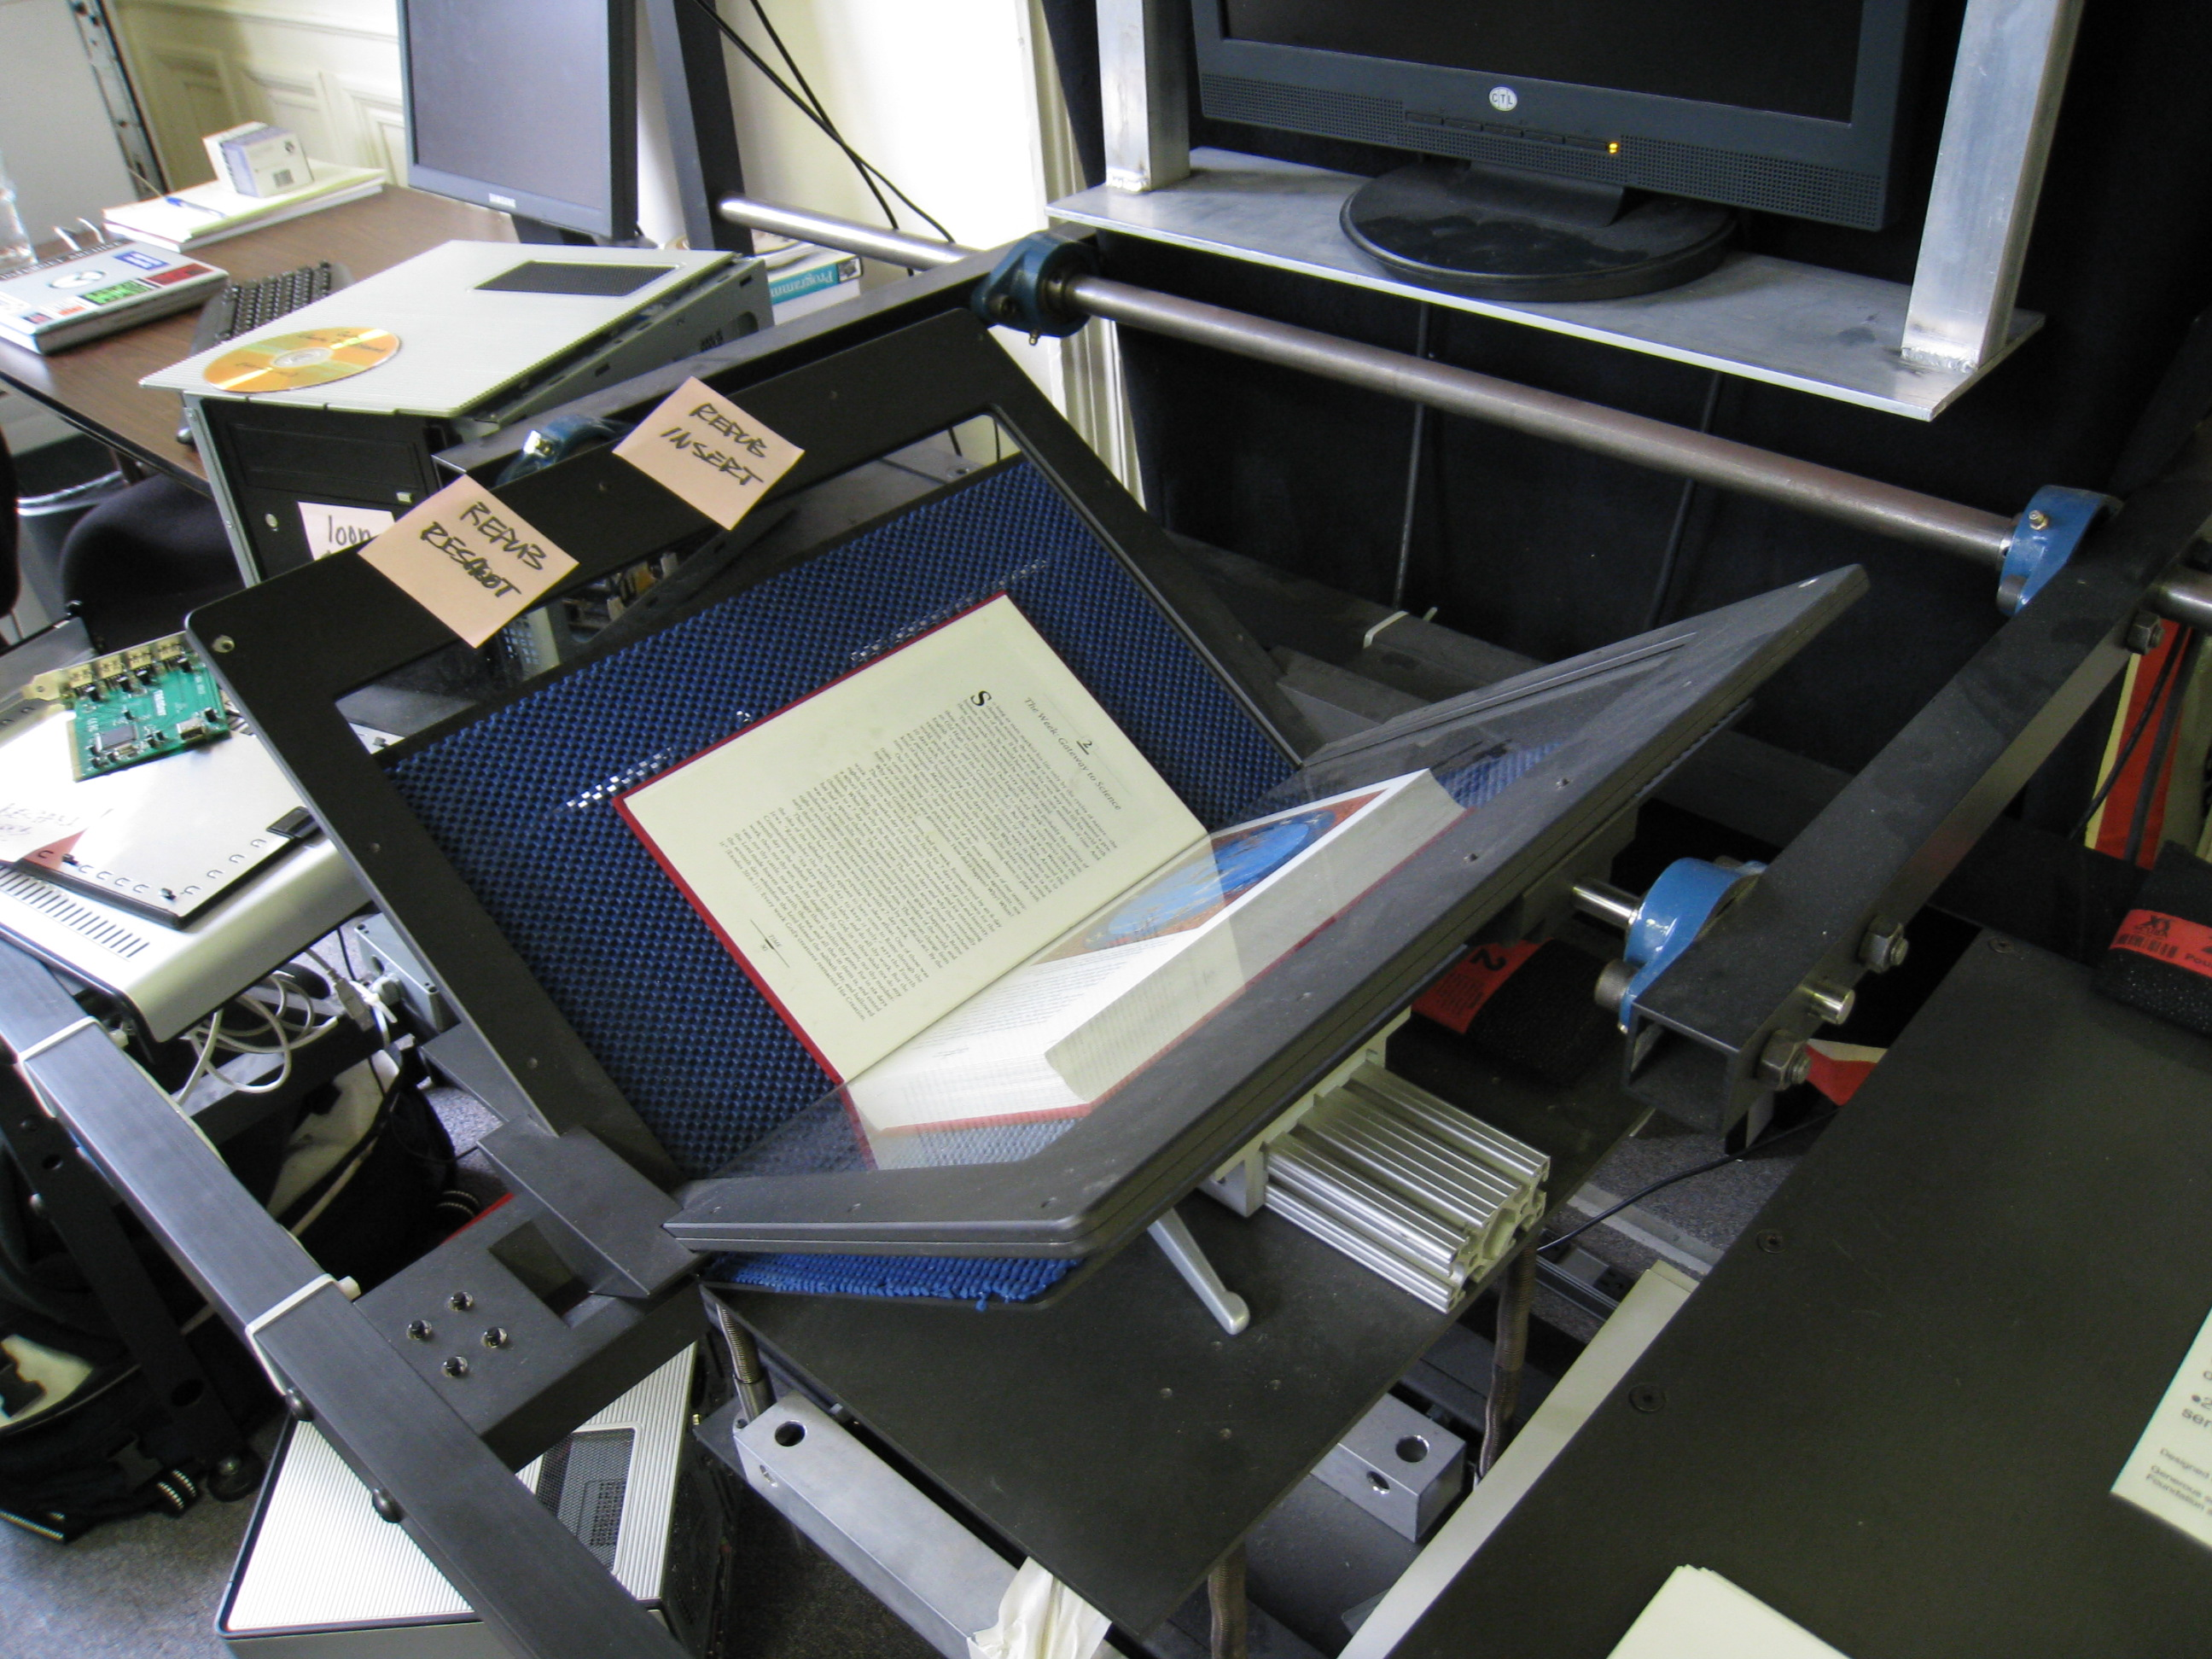
\includegraphics[width=0.7\textwidth]{fig/chapter1/Internet_Archive_book_scanner_1.jpg}
    \captionsetup{justification=centering}
    \caption{A book scanner at the Internet Archive headquarters in San Francisco, California}
    \label{ref:book_scanner}
\end{figure}

Despite their different goals with digitization, they rely the same types of technologies to achieve them. While simply scanning the books (see Figure \ref{ref:book_scanner}) will suffice to make the literature available online, other technologies are needed to actually index the content. Indexing is the process of capturing the scanned text and converting it into searchable data. To capture textual data, a technology called optical character recognition, or OCR for short, is used. OCR has many applications, and is in use in many areas today, such as book scanning, number plate recognition, handling of checks and passports, as well as assistive technologies for blind and visually impaired users \citep{mori1999optical, kurzweil2000reading}.

%%=========================================

\section{Problem and Motivation}
\label{sec:problem_motivation}
OCR is, in a broad sense, a branch of artificial intelligence, and a research branch in pattern recognition and computer vision \citep{mori1999optical}. It was first believed that it would be easy to develop an OCR, and researchers estimated that an accurate reading machine would be introduced in the 1950s. During the 1950s and the early 1960s researchers were still struggling with an ideal OCR model. Their early work has since laid the foundation for modern research in the field \citep{mori1992historical}. Things have progressed since the 1950s \citep{ye2015text}:

\begin{quote}
    While many researchers view optical character recognition (OCR) as a solved problem, text detection and recognition in imagery possess many of the same hurdles as computer vision and pattern recognition problems driven by lower quality or degraded data.
\end{quote}

OCR systems have reached great results, in some cases achieving up to 99\% recognition rates when working with clean and well-formatted documents under optimal conditions. However, in sub-optimal conditions, where the OCR system faces variants of text layouts and fonts, uneven illuminations, and other obstacles, the systems typically have notably lower rates of detection and recognition \citep{ye2015text}. Pasting of paper, ink spreading, fading, or dirt are just a few ways text can be damaged or obfuscated \citep{bhardwaj2014imaging}, which leads to obstacles and difficulties for OCR systems. In this thesis we take on a special kind of obfuscated text, and present a new way to recognize it by utilizing their ``signature''.

\subsection{Real World Example}
\begin{figure}[ht]
    \centering
    
\includegraphics[width=0.8\textwidth]{fig/chapter1/notch_tweet.jpg}
    \caption{Print screen of Tweet from notch}
    \label{ref:notch_twitter}
\end{figure}

An example of the type of obfuscated text we will attempt to handle in this thesis can be found in a Tweet from Markus ``Notch'' Persson. Persson is a Swedish video game programmer and designer, and is most famous for crating the highly acclaimed game Minecraft. He was an inveterate user of Twitter, and used to hint or tease upcoming features of the game. Figure \ref{ref:notch_twitter} contains a Tweet from Persson, which was Tweeted on June 12th 2011.

In this Tweet he is referring to an image which can be seen in Figure \ref{fig:notch_imgur}. It is a print screen of what looks like a text editor or IDE\footnote{Integrated Development Environment}. Although the image is heavily blurred and cropped, some of the text is still partially visible, like the lower portion of the file names in the tab pane at the top of the image. When this Tweet was posted, one user who called himself tmcaffeine on Reddit\footnote{\url{https://www.reddit.com}}, was able to identify the text in the tabs. He installed the same IDE Persson used, and matched the default font in the program against the letters that were partially visible in the image. His decoded image can be seen in in Figure \ref{fig:notch_eclipse_decoded}. More than four months later, when version 1.7 of Minecraft was released, it was clear that the decoding was correct as big mushrooms started to appear in the game\footnote{The experience orbs were postponed, and introduced in the 1.8 update instead.} \citep{misc-minecraft.172-changelog}.

\begin{figure}[h]
    \centering
    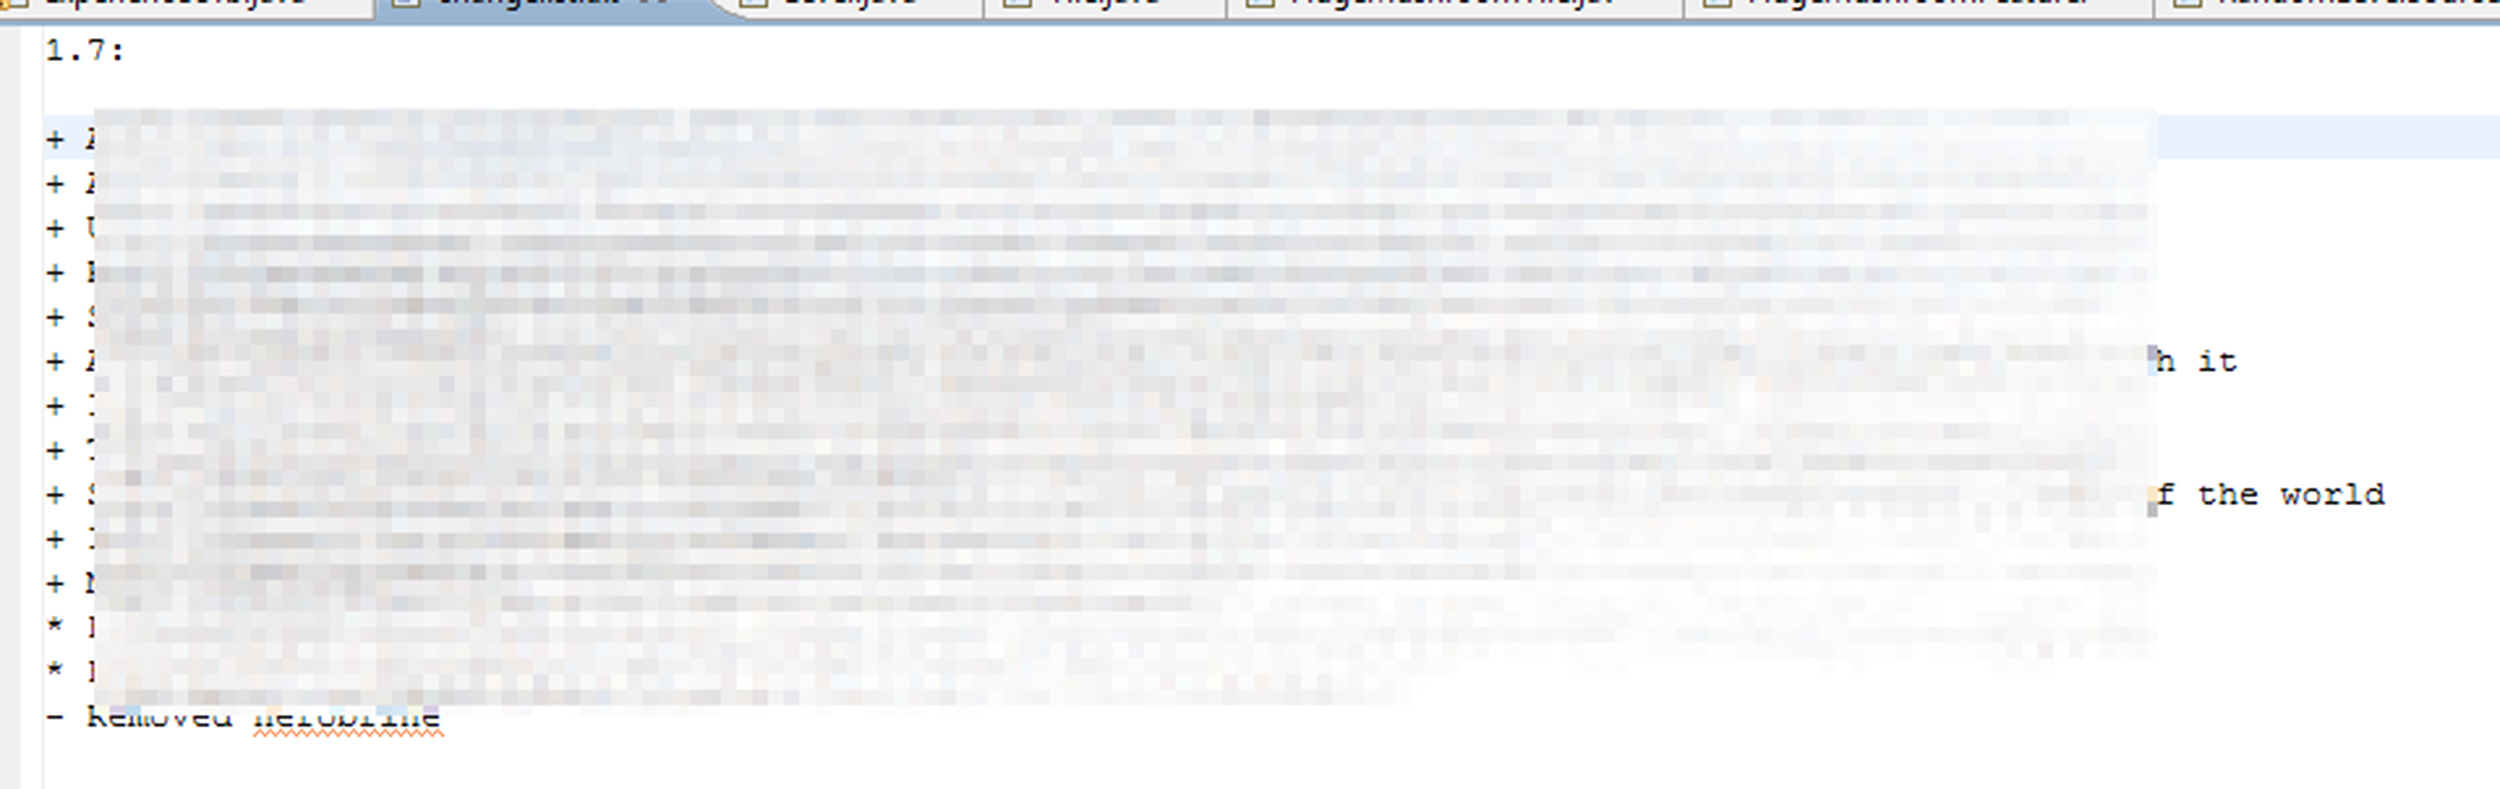
\includegraphics[width=0.8\textwidth]{fig/chapter1/notch_eclipse.jpg}
    \caption{Blurred image of @notch's changelog for Minecraft version 1.7}
    \label{fig:notch_imgur}
\end{figure}

\begin{figure}[ht]
    \centering
    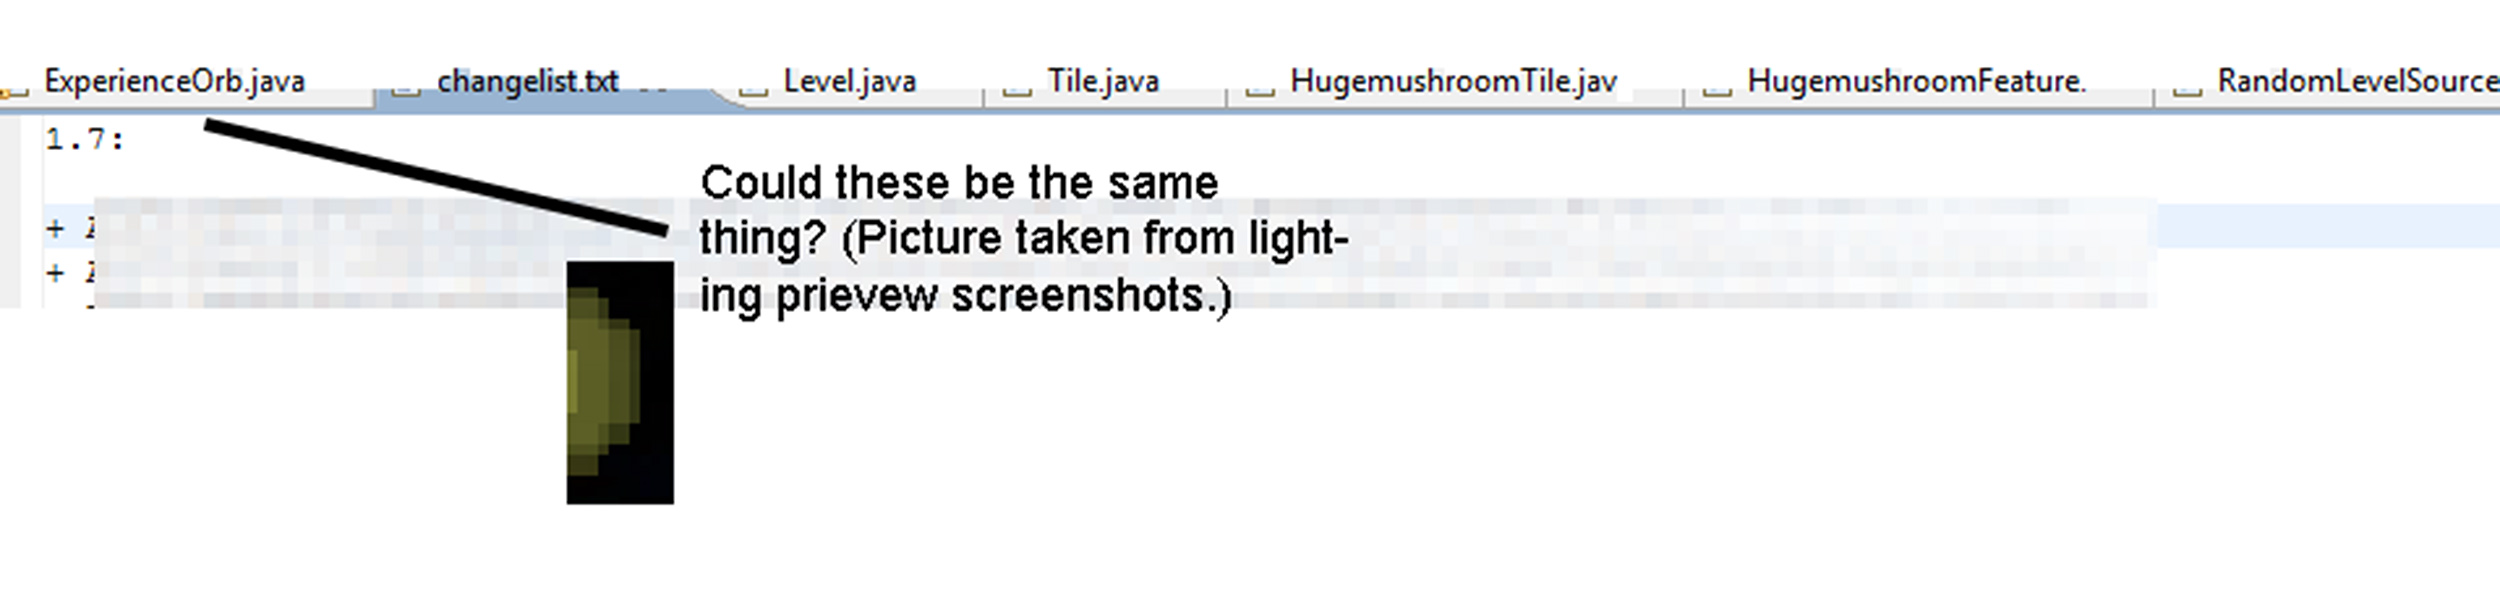
\includegraphics[width=0.8\textwidth]{fig/chapter1/notch_eclipse_decoded.jpg}
    \caption{Decoding of the blurred image from @notch's tweet done by Reddit user tmcaffeine}
    \label{fig:notch_eclipse_decoded}
\end{figure}

The decoding that was done to match the letters poses an interesting problem. Can characters and words be recognized given only a very small portion of the glyphs? The decoding in Figure \ref{fig:notch_eclipse_decoded} was done manually by comparing each letter with what was visible, but could such recognition be done automatically? Could such pattern recognition be learned? These questions were the basis for this thesis.

%%=========================================

\section{Goals and Research Questions}
\label{sec:goals_and_research_questions}
\begin{figure}[ht]
    \centering
    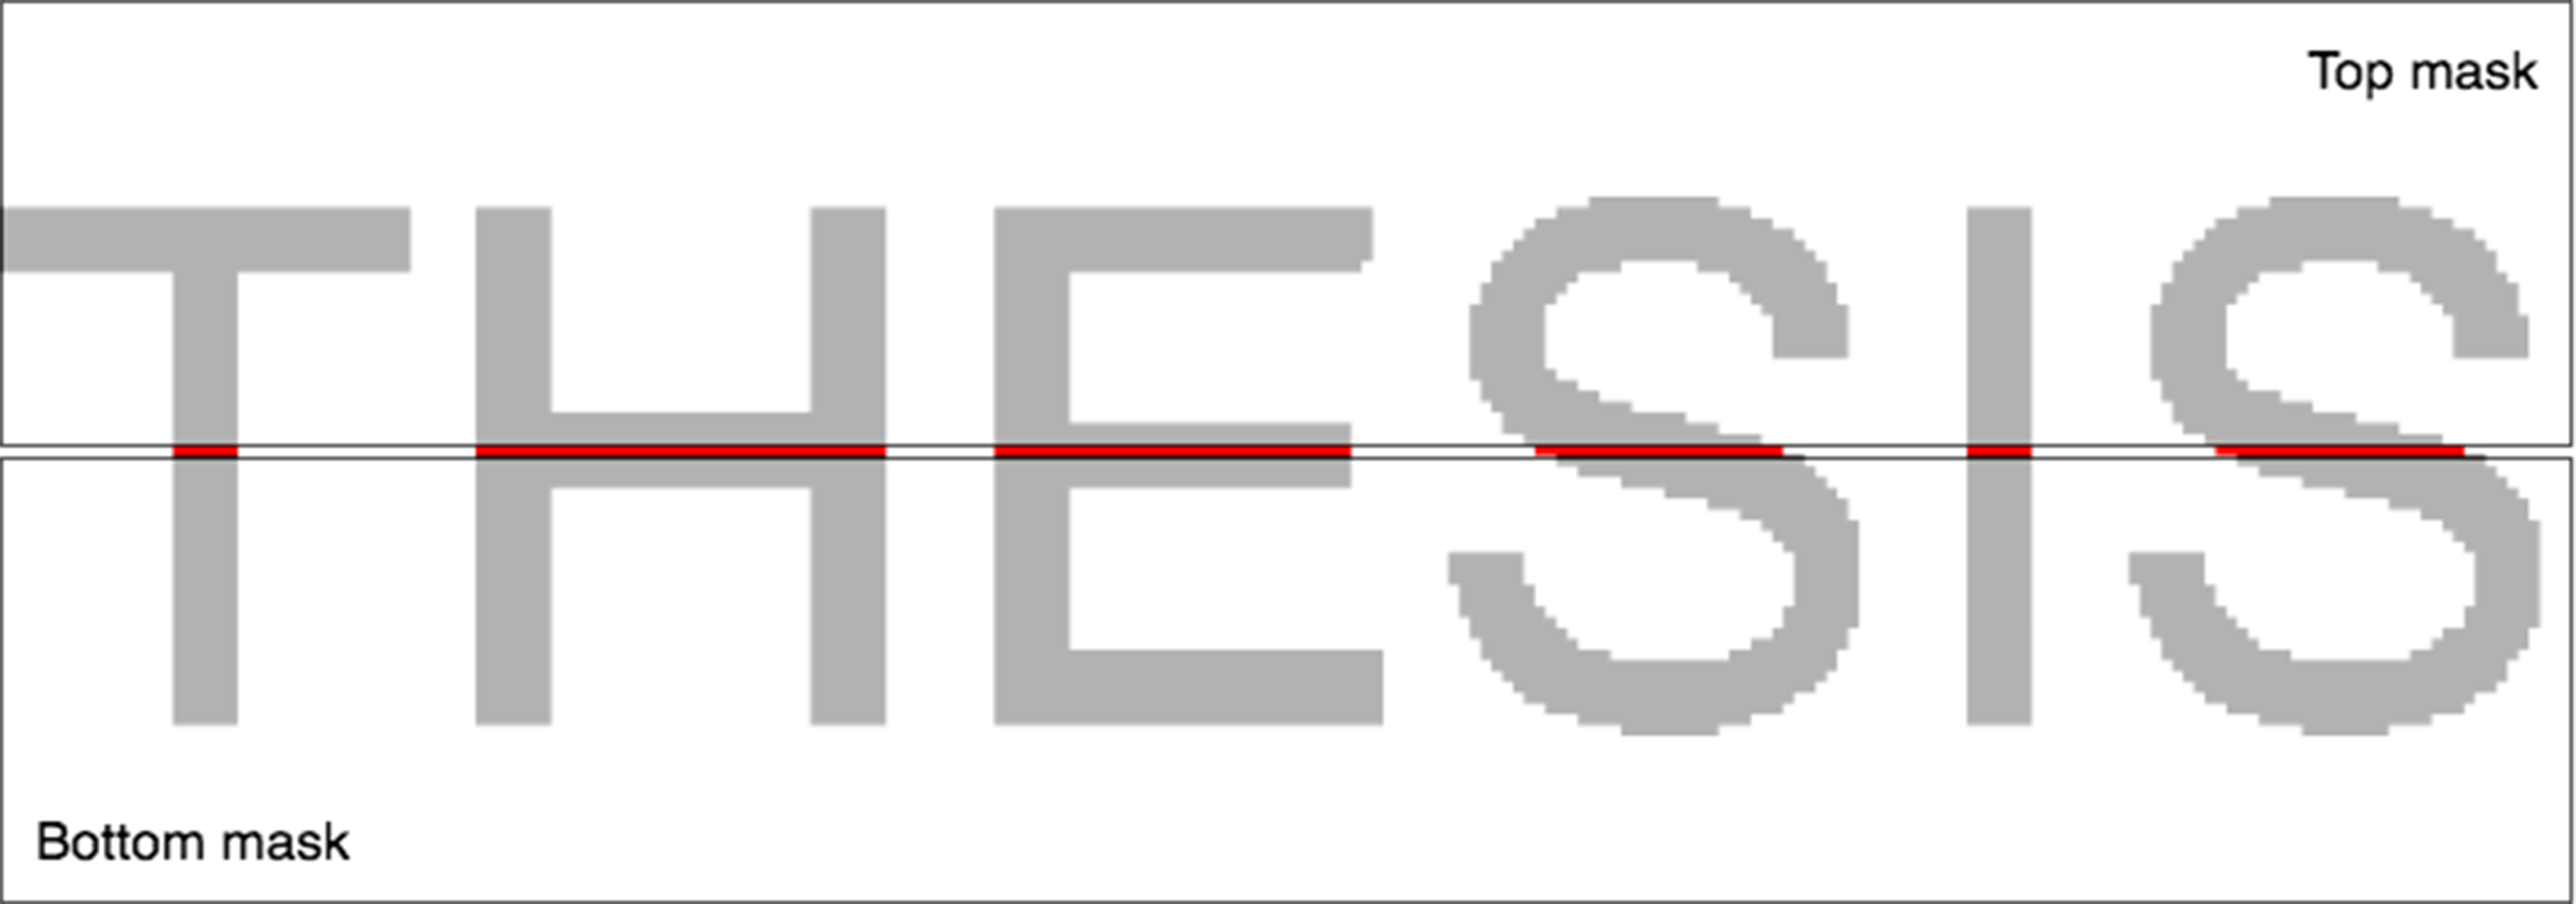
\includegraphics[width=1.\textwidth]{fig/chapter1/signature2.png}
    \caption{Illustration of a word with a signature with a height of one pixel}
    \label{fig:thesis-signature}
\end{figure}

Our goal is to use the ``signature'' of letters in a word to recognize it. We can imagine a ``signature'' by applying two masks to an image with some written text. These masks spans the total width of the image, and also cover most of the image from the top to bottom, and from the bottom to the top. The only area that is not covered by the masks is a thin line between the top and bottom masks. This line defines the ``signature'' for our image and the text written in it. 

Figure \ref{fig:thesis-signature} is an image with the word ``THESIS''. The original text in the image has a height of 50 pixels. Our masks are applied at both the top and bottom, exposing only a single line that has a height of one pixel. This line defines the ``signature'' for this word, and is highlighted in red. The areas that are covered by the masks are translucent and only shown for illustrative purposes. This is the approach we have used to extract signature sequences from machine-written words in this thesis.

Our overarching research goal is stated below. This was the main goal we focused on archiving throughout the work on this thesis. In addition to the research goal, we also created three research questions that we wanted to answer as well. Our research goal is somewhat open, and mainly explores whether or not an approach like the one we propose is possible or not, whereas the research questions are more specific and concrete. The research questions are asked to give get more insight and knowledge related to the approach we propose. The research questions and their meaning are explained in greater detail in Section \ref{sec:research_questions_and_approach}.

\begin{description}
    \item[Research Goal]{\textit{Develop a model that is able to use signature sequences to recognize words and letters}}
    \item[Research Question 1]{\textit{Does ambiguity in character signature sequences impact recognition rates?}}
    \item[Research Question 2]{\textit{Can a signature sequence based model handle multiple fonts at the same time?}}
    \item[Research Question 3]{\textit{Can a signature sequence based model be robust to noise?}}
\end{description}

%%=========================================

\section{Contributions}
\label{sec:contributions}
The contribution of this thesis is mainly the exploration of how to use machine learning and signature sequences to do recognition. The results of the experiments and conclusions done in this thesis may lay the foundation for new way to use machine learning to recognize patterns in data using sequences. Although the ideas presented in this thesis are not new, they may prove that certain problems can be solved using data in different ways. More detailed analysis and exploration in the underlying concepts and implementations of the models in context of our results will also serve as contributions. This may also give better insight in how the proposed models work and how they handle a problem with out characteristics.

%%=========================================

\section{Thesis Structure}
The remainder of this thesis is structured as follows:

\vspace{0.5cm}\noindent
\begin{minipage}{\linewidth}
    \textbf{{\hyperref[part1]{Part \ref{part1} -- \nameref{part1}}}}
    \begin{itemize}
        \item\textbf{\hyperref[ch:methodology]{Chapter \ref{ch:methodology} -- \nameref{ch:methodology}}} establishes the methodology used throughout the thesis. It explains how the research was carried out and how we chose our research approach.
    \end{itemize}
\end{minipage}

\vspace{0.5cm}\noindent
\begin{minipage}{\linewidth}
    \textbf{{\hyperref[part2]{Part \ref{part2} -- \nameref{part2}}}}
    \begin{itemize}
        \item\textbf{\hyperref[ch:problem]{Chapter \ref{ch:problem} -- \nameref{ch:problem}}} explains the problem in greater detail. It explains the various factors that defines our problem. We also look into how we can interpret out problem in context of established fields of machine learning. We also establish our method and approach to solve the problem.
        \item\textbf{\hyperref[ch:background]{Chapter \ref{ch:background} -- \nameref{ch:background}}} introduces some of the background information relevant to the proceeding chapter.
        \item\textbf{\hyperref[ch:related_work]{Chapter \ref{ch:related_work} -- \nameref{ch:related_work}}} presents related work done in the area of natural language processing, with a focus on machine translation. We present some of the earlier work as well as establishing state-of-the-art methods.
    \end{itemize}
\end{minipage}

\vspace{0.5cm}\noindent
\begin{minipage}{\linewidth}
    \textbf{{\hyperref[part3]{Part \ref{part3} -- \nameref{part3}}}}
    \begin{itemize}
        \item\textbf{\hyperref[ch:system_design]{Chapter \ref{ch:system_design} -- \nameref{ch:system_design}}} introduces the system we developed to run our experiments. This includes overall design and general approach, as well as key components.
        \item\textbf{\hyperref[ch:models]{Chapter \ref{ch:models} -- \nameref{ch:models}}} presents the three models we developed as a part of our research on basis of state-of-the-art technologies.
        \item\textbf{\hyperref[ch:experiments]{Chapter \ref{ch:experiments} -- \nameref{ch:experiments}}} establishes how we conducted our experiments, as well as presenting the structure of each experiment and what our goals and expectations were. This chapter also presents relevant configuration of the models, and choice of hyper-parameters.
    \end{itemize}
\end{minipage}

\vspace{0.5cm}\noindent
\begin{minipage}{\linewidth}
    \textbf{{\hyperref[part4]{Part \ref{part4} -- \nameref{part4}}}}
    \begin{itemize}
        \item\textbf{\hyperref[ch:results]{Chapter \ref{ch:results} -- \nameref{ch:results}}} presents the results for each experiment explained in the previous chapter, followed by discussion the results and evaluation the models. We also analyze the models in the context of the results from the experiments.
        \item\textbf{\hyperref[ch:conclusion]{Chapter \ref{ch:conclusion} -- \nameref{ch:conclusion}}} draws the conclusion for our work. We state our research contribution, and present thoughts on possible paths for future work.
    \end{itemize}
\end{minipage}